\cleardoublepage

\section{研究区域与数据}
\subsection{研究区概况}
\par 据联合国粮食与农业组织(FAO)统计,2022年中国玉米产量已占全球23.9\%,位居世界第二,同时中国也是世界两大玉米消费国之一,占全球消费总量的25.2\%。因此,玉米生产不论在区域经济还是在全球食品安全方面都有着重要意义。
\par 目前,我国的玉米种植分布极不均衡,主要集中于东北、华北与西南地区。其中,2022年东北三省的玉米产量占全国总产量的34.3\%。东北地区作为中国主要的粮食生产基地,其中的东北平原耕地广阔,地势平坦,利用遥感手段提取作物生长信息较为便利。因此,研究选定东北三省作为研究区域,即黑龙江省、吉林省与辽宁省,该地区以旱地为主,采用一季耕作模式,每年4-5月播种,9-10月收获。

\subsection{作物数据}
\par 在本研究中,东北地区各地级市的玉米总产量数据来源于知网中国经济社会大数据研究平台提供的黑龙江省、吉林省和辽宁省的统计年鉴。经过数据合并和清洗,获得了2000年至2019年东北地区地级市的玉米总产量数据。在数据处理过程中,注意到黑龙江省在2013年至2018年期间单独统计了绥芬河市和抚远市的作物总产量数据。因此,在对数据进行合并时,将这两个城市的产量数据分别合并入牡丹江市和佳木斯市的玉米总产量中,便于后续进行统一计算。

\par 东北三省的县级玉米总产量数据来源于1981年至2012年的全国区县主要作物统计数据。通过对这些数据进行筛选和清洗,仅保留黑龙江省、吉林省和辽宁省的区县数据,研究获取了2000年至2012年的东北地区县级玉米总产量。

\subsection{遥感数据}
\par 中分辨率成像光谱仪(MODIS)是由美国宇航局(NASA)研发制造的一种空间遥感仪器,可以连续监测全球光谱数据,包括陆地、海洋与大气特征。这种仪器搭载于 Terra 和 Aqua 两颗卫星,通过1-2天一次对地球进行观测,结合多种算法,可以提供多种高时间、高空间分辨率的地球观测数据。MODIS可以提供多种数据产品,如气溶胶、云、地表温度、地表覆盖和生态系统动态等。这些数据产品被广泛应用于农业、森林、水资源、环境和气候变化等多个领域的研究。

\par 借助 MODIS 产品可以监测陆地表面的植被生长和物候期变化。在本研究中,地表反射率数据使用MOD09A1 V6.1产品,该产品提供了Terra MODIS 1-7波段的地表反射率估计值,对气体、气溶胶以及瑞利散射等大气条件进行了矫正。叶面积指数数据使用MOD15A2H V6.1产品,产品提供了叶面积指数(LAI)和光合有效辐射分数(FPAR),选择Terra传感器连续8天内的最佳数据作为像素值。地表蒸发量数据来源于MOD16A2 V6产品,该产品为结合了蒸发量和潜热通量的综合产品,像素值为观测期内的数值总和。此外,还选用了总初级生产力数据,来源于MOD17A2H V6,该产品的像素值由观测期内的数据累积得到。以上遥感产品空间分辨率均为500m,时间分辨率均为8天。上述MODIS产品的数据波段分布与数值范围情况如\autoref{tab:modis}所示。

\begin{table}
  \centering
  \caption{MODIS数据波段分布}
  \label{tab:modis}
  \begin{tabularx}{\linewidth}{cX<{\centering}X<{\centering}X<{\centering}}
      \toprule
      MODIS产品 & 波段名称 & 光谱范围 & 数值范围 \\
      \midrule
      & sur\_refl\_b01 & 620-670nm & (-100, 16000) \\
      & sur\_refl\_b02 & 841-876nm & (-100, 16000) \\
      & sur\_refl\_b03 & 459-479nm & (-100, 16000) \\
      MOD09A1 & sur\_refl\_b04 & 545-565nm & (-100, 16000) \\
      & sur\_refl\_b05 & 1230-1250nm & (-100, 16000) \\
      & sur\_refl\_b06 & 1628-1652nm & (-100, 16000) \\
      & sur\_refl\_b07 & 2105-2155nm & (-100, 16000) \\ \hline
      MOD15A2H  & Lai\_500m & / & (0, 100) \\ \hline
      MOD16A2   & ET & / & (-32767, 32700) \\ \hline
      MOD17A2H  & Gpp & / & (0, 3000) \\
      \bottomrule
  \end{tabularx}
\end{table}

\subsection{物候分布数据集}
\par 研究中所用玉米分布数据来源于张朝等人制作的2000-2019年我国三大粮食作物物候分布图 ChinaCropPhen1km\cite{luo2020chinacropphen1km},该产品空间分辨率为1km,其中玉米种植被分为了发芽期(HE)、V3阶段(V3)和成熟期(MA)。数据集可通过Figshare平台(https://figshare.com)获取。

\subsection{数据预处理}
\par 在获取MODIS产品数据方面,目前主要使用谷歌云计算平台(Google Earth Engine, GEE)提供的云计算服务\cite{gorelick2017google}。平台数据目录存放了大量可公开获取的地理空间数据集,并可以通过基于Javascript API的Web端或Python API进行批量数据处理,能够满足各种研究需求。GEE 通过自身高效的计算能力和较为完整且实时更新的地理空间数据集,帮助用户通过统一简洁的编程环境对数据进行预处理操作,高效地解决了不同来源数据集在获取与处理过程中带来的处理时间冗长与存储空间不足问题。

\par 介于以上优点,研究使用了 GEE 平台提供的 Python API,并结合 Shell 和 Python 脚本,批量获取了2000年到2019年18年内4月1日至10月31日的四项产品数据。这些数据分别被划分至地级市尺度和区县尺度,利用全国行政区划矢量数据进行划分。为了方便后续处理,将这些数据在云端先重采样至1km,再下载到本地进行进一步的处理和分析。同理,利用已有的行政区划数据对 ChinaCropPhen1km 数据集进行分割,并按照年份和行政区域分别对其进行存储。

\par 地理空间数据抽象库\cite{warmerdam2008geospatial}(Geospatial Data Abstraction Library, GDAL)是一个开源地理空间数据处理库,它提供了一套完整的工具集,可用于读取、写入、转换和分析各种地理空间数据格式。通过使用 GDAL 对 ChinaCropPhen1km 数据集进行重投影处理,可以将其与 MODIS 产品数据进行匹配,以准确提取玉米种植地区的遥感信息。此外,将两数据集进行掩膜计算可以实现仅保留玉米种植地区的遥感信息,从而排除了其他不相关的信息干扰的目的。通过重投影与掩膜计算,研究成功获得了2000年至2019年地级市尺度以及2000年至2012年区县尺度的玉米遥感特征数据集。

\par 经过数据预处理后,遥感特征数据集可以如\autoref{equ:modis_series}所示:

\begin{equation}
    \label{equ:modis_series}
    I=(I^1, I^2, ..., I^t, ..., I^T), I^t\in R^{r\times c\times b}
\end{equation}
\par 其中,$I^t$指时间$t$时的多波段遥感影像;$r$、$c$、$b$分别指影像的行数、列数和波段数;$T$指影像的时间序列长度。在本研究中,$T=26$,$b=10$。

\section{研究方法}
\subsection{估产样本构建}

\par 通过上述数据预处理步骤,可以获得如\autoref{equ:dataset1}所示的样本数据集:

\begin{equation}
  \label{equ:dataset1}
  D=\{(I_1, y_1),(I_2, y_2), ..., (I_n, y_n)\}
\end{equation}

\par 其中,$y$为地区总产量,每一个样本$(I_t, y_t)$表示了某地区某年份的玉米遥感特征影像和总产量。

\par 为了降低样本数据的维度,研究采用直方图降维的方法对样本数据进行降维处理。直方图降维的前提是假设玉米产量与像素空间分布无关,仅与不同像素数量相关。为确定直方图降维范围,减少直方图降维过程中的信息损失,研究首先借助 GDAL 库对各个波段的最大、最小值进行获取,统计了玉米特征样本集中像素值范围,如\autoref{tab:range}所示:

\begin{table}
  \centering
  \caption{MODIS数据波段范围}
  \label{tab:range}
  \begin{tabularx}{\linewidth}{cX<{\centering}X<{\centering}}
    \toprule
    MODIS产品 & 波段名称 & 数值范围 \\
    \midrule
    & sur\_refl\_b01 & (44, 9397) \\
    & sur\_refl\_b02 & (67, 9046) \\
    & sur\_refl\_b03 & (4, 9064) \\
    MOD09A1 & sur\_refl\_b04 & (36, 9239) \\
    & sur\_refl\_b05 & (37, 8148) \\
    & sur\_refl\_b06 & (60, 6767) \\
    & sur\_refl\_b07 & (-14, 6184) \\ \hline
    MOD15A2H  & Lai\_500m & (0, 116) \\ \hline
    MOD16A2   & ET & (0, 670) \\ \hline
    MOD17A2H  & Gpp & (0, 986) \\
    \bottomrule
\end{tabularx}
\end{table}

\par 借助于\autoref{tab:range}中的数值范围,研究将每个波段的像素值划分为$bins$个范围。在本研究中,10个波段的阈值被分别设置为:(0, 9400)、(0, 9100)、(0, 9100)、(0, 9300)、(0, 8200)、(0, 6800)、(0, 6600)、(0, 120)、(0, 700)、(0, 1000)。将每个波段的像素值进行直方图统计,同时对生成的像素直方图进行如\autoref{equ:normalize}所示的方式进行归一化处理,最终得到每个波段的直方图。

\begin{equation}
  \label{equ:normalize}
  M^t_{i}=\frac{M^t_{i}}{\sum_{i=1}^{bins}M^t_{i}}
\end{equation}

\par 每个样本的特征向量表示如\autoref{equ:histogram}所示,其中,$M^t$指时间$t$时的多波段直方图,$bins$、$b$分别指直方图的行数、波段数。在本研究中,$bins=64$,$b=10$。

\begin{equation}
  \label{equ:histogram}
  M=(M^1, M^2, ..., M^T), M^t\in R^{bins\times b}
\end{equation}

\par 经过直方图降维与归一化处理,样本集表示为如\autoref{equ:dataset2}所示,$(M_t, y_t)$表示了某地区某年份的单个样本,其中$M_t$是形状为$64\times 26\times 10$的玉米遥感特征向量,$y_t$为玉米总产量。

\begin{equation}
  \label{equ:dataset2}
  D=\{(M_1, y_1),(M_2, y_2), ..., (M_n, y_n)\}
\end{equation}

\par 在本次实验中,东北地区地级市尺度玉米样本集包含2002年-2019年东北地区36个地级市646个样本,其中538个样本作为训练集,108个样本作为测试集;区县级尺度玉米样本集包含2002年-2012年282个区县的2335个有效样本,其中1850个样本作为训练集,485个样本作为测试集。

\subsection{模型构建}
\subsubsection{结合注意力机制的长短期记忆神经网络}

\par 研究使用的深度学习网络由两部分组成,如\autoref{fig:network}所示,首先由两个LSTM层分别接收由地表反射率共7个波段降维得到的特征向量和由地表蒸发量、叶面积指数和总初级生产力共3个波段降维得到的特征向量。通过将两个隐藏层的输出进行拼接,输入至注意力层计算参数权重向量,与原有特征向量进行乘计算后获得最终的特征向量。最后,特征向量经过三个全连接层,输出最终的玉米总产量预测值。

\begin{figure}[ht]
  \centering
  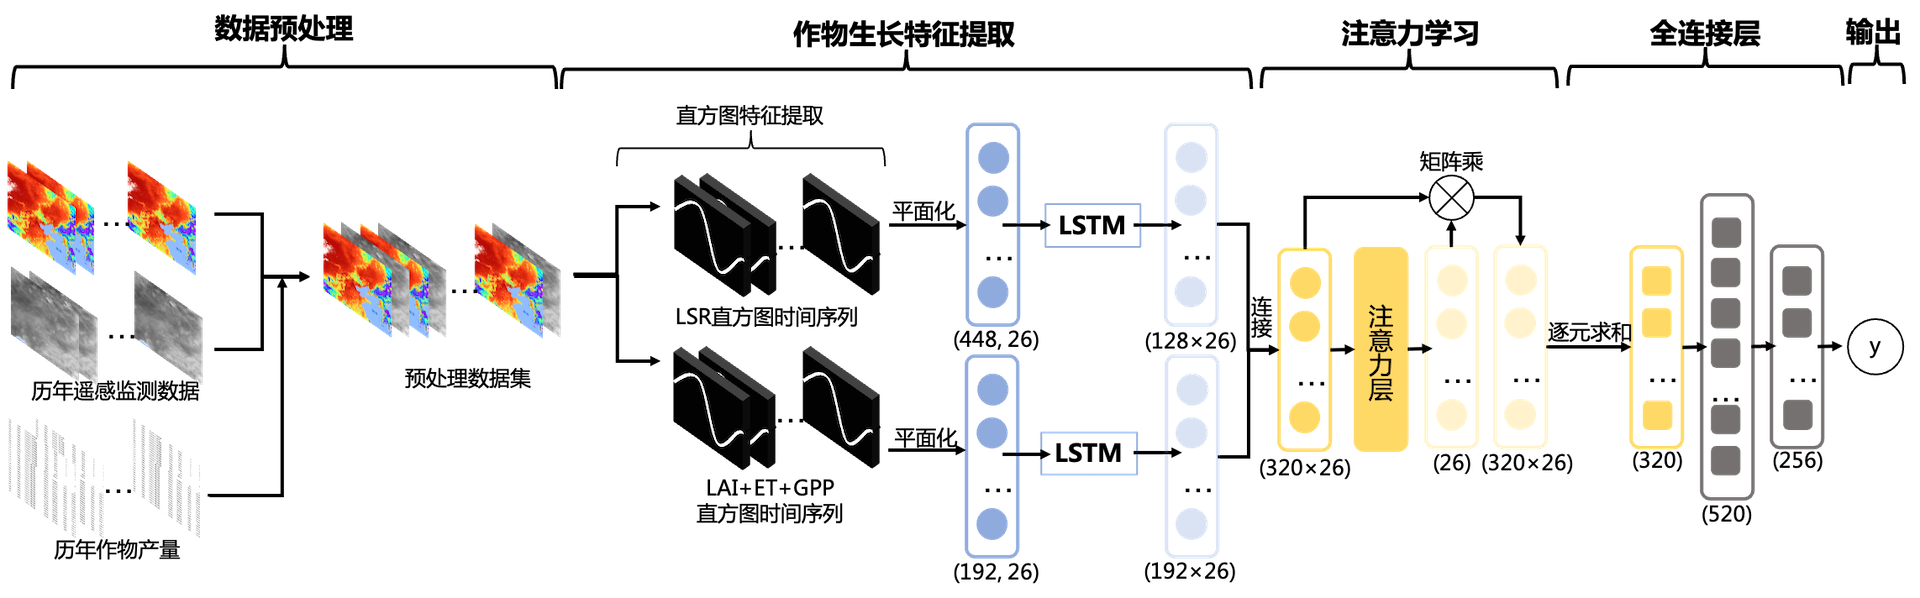
\includegraphics[width=\linewidth]{network.png}
  \caption{\label{fig:network}研究网络结构}
\end{figure}

\par 长短期记忆神经网络(LSTM)作为一种特殊的循环神经网络(RNN),通过引入额外的“记忆单元”和门控机制,能够更好地捕捉和处理时间序列中的信息与关系\cite{LI2019104785}。在每个时间步骤$t$,LSTM的输入$x_t$会被送到sigmoid激活的“输入门”$g_i^t$中,控制是否要更新单元状态$C_t$。由另一个sigmoid激活的“遗忘门”$g_f^t$决定是否保留以前的单元状态$C_{t-1}$。通过应用输入门和遗忘门的计算值,计算得到当前的单元状态$C_t$。在本研究中,对于输出的隐藏状态序列$\{h^1, h^2, ..., h^T\}$,$h^t$的计算过程如下:

\begin{equation}
  \label{equ:lstm1}
  g_f^t=\sigma (W_f\cdot [h^{t-1}, x^t]+b_f)
\end{equation}
\begin{equation}
  \label{equ:lstm2}
  g_i^t=\sigma (W_i\cdot [h^{t-1}, x^t]+b_i)
\end{equation}
\begin{equation}
  \label{equ:lstm3}
  C^t=g_f^t\cdot C^{t-1}+g_i^t\cdot tanh(W_c\cdot [h^{t-1}, x^t]+b_c)
\end{equation}
\begin{equation}
  \label{equ:lstm4}
  g_o^t=\sigma (W_o\cdot [h^{t-1}, x^t]+b_o)
\end{equation}
\begin{equation}
  \label{equ:lstm5}
  h^t=g_o^t\cdot tanh(C^t)
\end{equation}

\par 其中$W_c$、$W_i$、$W_f$、$W_o$、$b_c$、$b_i$、$b_f$和$b_o$分别是细胞状态更新、输入门、遗忘门和输出门的权重矩阵(W)和偏置向量(b)。$g_f^t$、$g_i^t$和$g_o^t$分别是这些门产生的向量。三个向量的取值范围为$[0,1]$,其中0代表完全删除信息,1代表完全保存信息。本研究中,采用了两个并列的LSTM层,分别使用128和192个隐藏单元。

\par 注意力机制是一种用于提取序列中重要信息的机制,能够帮助模型更好地捕捉序列中的信息,提高模型的泛化能力。而已有研究表明,玉米种植过程中不同时间段环境因素对玉米最终总产量的影响程度有所不同\cite{shook2021crop}。因此,研究在LSTM层的输出上添加注意力机制层,通过使用全连接层和softmax激活为每个隐藏特征$h^t$产生了注意力权重$\alpha ^t$,$\alpha ^t$的计算方式如\autoref{equ:attention_alpha}所示。

\begin{equation}
  \label{equ:attention_alpha}
  \alpha ^t=softmax (W_a\cdot h^t+b_a)
\end{equation}

\par 最终,注意力权重$\{\alpha ^1,\alpha ^2,..., \alpha ^T \}$与隐藏特征$\{h ^1,h ^2,..., h ^T \}$相乘,得到最终的特征向量:

\begin{equation}
  \label{equ:attention}
  H=\sum_{t=1}^T \alpha ^t\cdot h^t
\end{equation}

\par 最后,特征向量将依次经过神经元数量为512、256和1的三个全连接层。其中,每个全连接层都包含了批归一化(BatchNormalize, BN)层、ReLu激活层和Dropout层,随机失活率被分别设定为40\%、20\%和0\%,最终输出最终的玉米总产量预测值。

\par 在模型训练过程中,损失函数选定为L2损失函数;优化器选择了 Adam 优化器;学习率初始值为0.0001;批次大小(Batch Size)为32。

\subsubsection{对比模型}

\par 为了验证提出模型的有效性,研究还对比了三个基准模型,分别是 LSTM 模型、 CNN 模型和随机森林(RF)模型。

\par LSTM 模型分为两种:单层 LSTM 模型和包含两个并列 LSTM 的模型,同时,为证明注意力机制的有效性,对比模型中分别加入了不包含注意力机制层的两种LSTM模型。

\par CNN 模型借鉴了由 You 等人\cite{you2017deep}提出的卷积神经网络结构,包含六个卷积层C1~C6,卷积核个数分别为64、64、128、128、256和256,卷积核大小均为$3\times 3$,滑动步长分别为2、1、2、1、2和1。每个卷积层后面都包含一个批归一化层和一个ReLu激活层。最后,将卷积层的输出依次经过神经元数量为512、256和1的三个全连接层,每个全连接层后的 Dropout 参数分别为50\%、30\%和20\%,最终输出玉米总产量预测值。

\par 对于随机森林模型,研究采用了 sklearn 库中的 RandomForestRegressor 类,该类实现了一种基于随机森林的回归算法。在随机森林模型的训练过程中,通过设置了多个关键参数,确保模型的稳定性和准确性。其中,随机森林中树的数量为200,树的最大深度为8,每个节点的最小样本数为3,每个叶子节点的最小样本数为4。

\subsection{评价指标}

\par 为了评价模型的预测效果,研究采用了决定系数($R^2$)、均方根误差(RMSE)和皮尔森相关系数(Pearson's R)三个评价指标。其中,$R^2$衡量了模型解释数据方差的能力,其值越接近1,表示模型对数据的解释越好。RMSE 用于度量模型预测值和实际值之间的误差大小,其值越小,表示模型预测的准确性越高。Pearson's R 用于评估模型输出和真实值之间的线性相关性,其值介于-1到1之间。其具体计算公式表示如下:

\begin{equation}
  \label{equ:R2}
  R^2=1-\frac{\sum_{i=1}^n (y_i-\hat{y}_i)^2}{\sum_{i=1}^n (y_i-\bar{y}_i)^2}
\end{equation}
\begin{equation}
  \label{equ:RMSE}
  RMSE=\sqrt{\frac{\sum_{i=1}^n (y_i-\hat{y}_i)^2}{n}}
\end{equation}
\begin{equation}
  \label{equ:Pearson}
  Pearson's R=\frac{\sum_{i=1}^n (y_i-\bar{y}_i)(\hat{y}_i-\bar{\hat{y}}_i)}{\sqrt{\sum_{i=1}^n (y_i-\bar{y}_i)^2}\sqrt{\sum_{i=1}^n (\hat{y}_i-\bar{\hat{y}}_i)^2}}
\end{equation}

\par 其中,$y_i$表示第i个样本的真实总产量,$\hat{y}_i$表示第i个样本的预测总产量,$\bar{y}_i$表示第i个样本真实平均总产量,$\bar{\hat{y}}_i$表示第i个样本预测平均总产量,$n$为样本总数。


\section{结果分析}
\subsection{估产精度分析}
\par 研究构建的玉米估产模型与对比估产模型评价指标如\autoref{tab:score_city}和\autoref{tab:score_county}所示。在实验中,地级市尺度的模型测试选取了2017年-2019年三个年份不同城市的样本数据;县级尺度的估产模型选取了2012年的样本数据进行测试。结果显示,结合了注意力机制且包含两个LSTM层输入的 DUAL\_ATT 模型拥有最好的估产精度,在决定系数$R^2$、均方根误差 RMSE 和皮尔森相关系数 Pearson's R 三个指标上,均优于其他模型。

\begin{table}
  \centering
  \caption{各地级市尺度玉米估产模型精度评价}
  \label{tab:score_city}
  \begin{tabularx}{\linewidth}{cX<{\centering}X<{\centering}X<{\centering}}
      \toprule
      模型 & $R^2$ & RMSE(万吨) & Pearson's R \\
      \midrule
      DUAL\_ATT & 0.8244 & 101.2051 & 0.9112 \\
      LSTM\_ATT & 0.7182 & 128.2270 & 0.8831 \\
      DUAL & 0.7561 & 119.2947 & 0.8935 \\
      LSTM & 0.6896 & 134.5782 & 0.8508 \\
      CNN & 0.6221 & 148.4906 & 0.8735 \\
      RF & 0.6409 & 144.7494 & 0.8557 \\ 
      \bottomrule
  \end{tabularx}
\end{table}

\begin{table}
  \centering
  \caption{各县级尺度尺度玉米估产模型精度评价}
  \label{tab:score_county}
  \begin{tabularx}{\linewidth}{cX<{\centering}X<{\centering}X<{\centering}}
      \toprule
      模型 & $R^2$ & RMSE(万吨) & Pearson's R \\
      \midrule
      DUAL\_ATT & 0.6141 & 39.4236 & 0.8214 \\
      LSTM\_ATT & 0.5255 & 43.7140 & 0.7318 \\
      DUAL & 0.4847 & 45.5544 & 0.7767 \\
      LSTM & 0.5578 & 42.1994 & 0.8131 \\
      CNN & 0.3369 & 55.4357 & 0.7089 \\
      RF & 0.2933 & 56.9983 & 0.7441 \\ 
      \bottomrule
  \end{tabularx}
\end{table}

\par 可以看出,研究采用的玉米估产模型对于区域总产量预测具有较高的准确性。该模型通过直方图降维和归一化方法进行特征提取,减少了信息损失。通过与双层 LSTM 和注意力机制结合,该模型能够更好地捕捉时间序列信息,有效地拟合了作物生长的复杂过程。然而,模型在采用了 Dropout 层、批归一化层以及 L2 参数正则化方法之后,仍然出现了训练集的预测精度相比验证集更高的过拟合现象。这表明模型训练样本较少,增加训练样本数量有助于提高模型的预测精度。

\par 与其他地级市尺度的玉米估产模型相比,卷积神经网络模型(CNN)和随机森林模型(RF)表现相对不理想。这可能是由于这些模型处理存在时间序列的数据的能力有所不足,无法捕捉到作物生长的复杂过程。实验中简单的长短期记忆神经网络(LSTM)较好的性能也体现了挖掘作物生长的时序信息在玉米总产量预测中的重要性,这也在DUAL\_ATT模型中得到了体现。与LSTM\_ATT、DUAL两种模型相比,DUAL\_ATT模型在估产结果上有着更好的精度,这也分别表明了注意力机制和双层 LSTM 引入的有效性。

\par 然而可以注意到,在区县尺度玉米估产模型的测试中,所有测试模型的表现均不如地级市尺度的模型。这可能是由于区县尺度的玉米总产量数据分布较为不均匀,如\autoref{fig:hist}所示,在将东北地区划分为区县尺度后,样本区域内玉米分布面积普遍偏少,这导致模型在区县尺度上难以有效提取作物生长过程中的特征,预测精度降低。此外,由于区县尺度下作物产量数据获取难度较大,数据的精度、广度均有所不足,也导致了模型在区县尺度上表现不佳。

\begin{figure}
  \centering
  \subcaptionbox{地级市尺度玉米面积分布}[.5\linewidth]{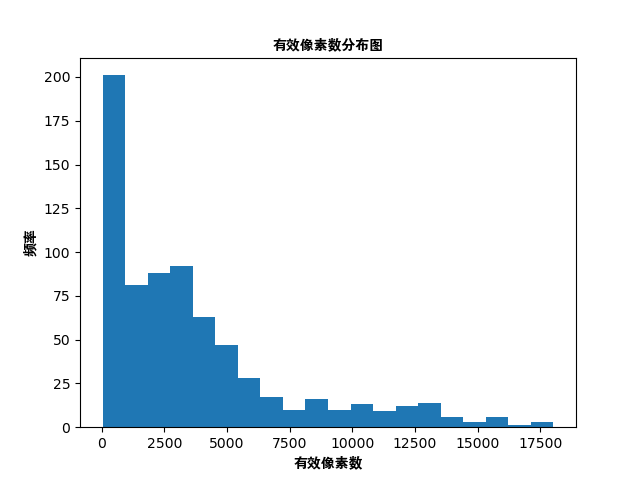
\includegraphics[width=.8\linewidth]{result/hist_city.png}}\hfill
  \subcaptionbox{区县尺度玉米面积分布}[.5\linewidth]{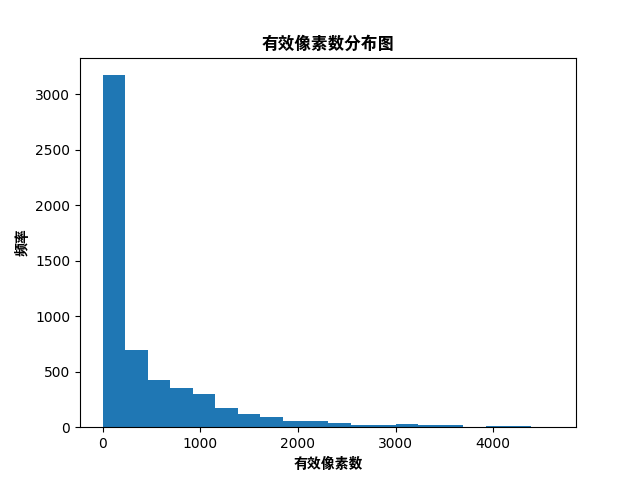
\includegraphics[width=.8\linewidth]{result/hist_county.png}}\hfill
  \caption{样本集玉米种植面积分布}
  \label{fig:hist}
\end{figure}

\par 各估产模型预估产量与实际产量的散点图如\autoref{fig:scatter_city}和\autoref{fig:scatter_county}所示。可以观察到,在各估产模型中,区县尺度的作物估产模型更容易低估玉米总产量值。这可能是由于区县尺度下玉米种植面积普遍较小,导致预测高产量区域的玉米产量较为困难,从而导致了模型在区县尺度下的低估现象。此外,由于模型输入参数仅包含了如地表反射率、叶面积指数、地表蒸发量与总初级生产力等反映在作物生长特征的数据,并没有考虑到农业生产技术的进步导致作物单产的提升,这给产量预测带来了较大的困难。该尺度下,使用结合注意力机制和双层 LSTM 的 DUAL\_ATT 模型能一定程度地缓解低估现象,然而模型仍会受到上述因素的影响,导致模型在区县尺度下低估高产量区域的玉米总产量。

\begin{figure}
  \centering
  \subcaptionbox{DUAL\_ATT}{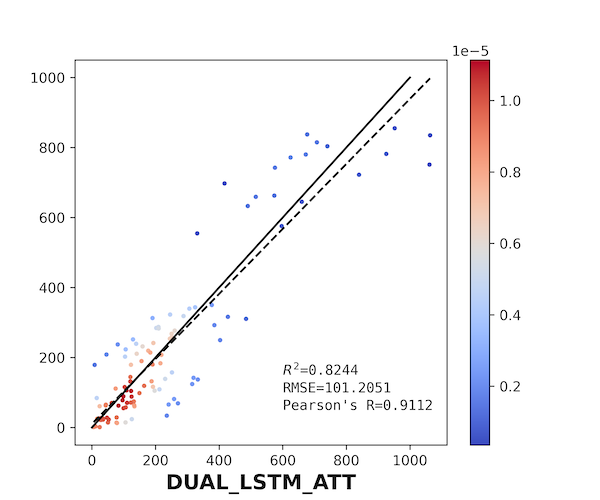
\includegraphics[width=.3\linewidth]{result/dual_att_city.png}}\hfill
  \subcaptionbox{LSTM\_ATT}{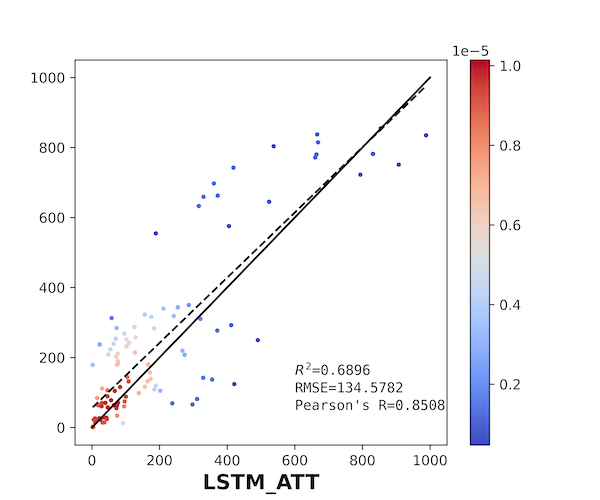
\includegraphics[width=.3\linewidth]{result/lstm_att_city.png}}\hfill
  \subcaptionbox{CNN}{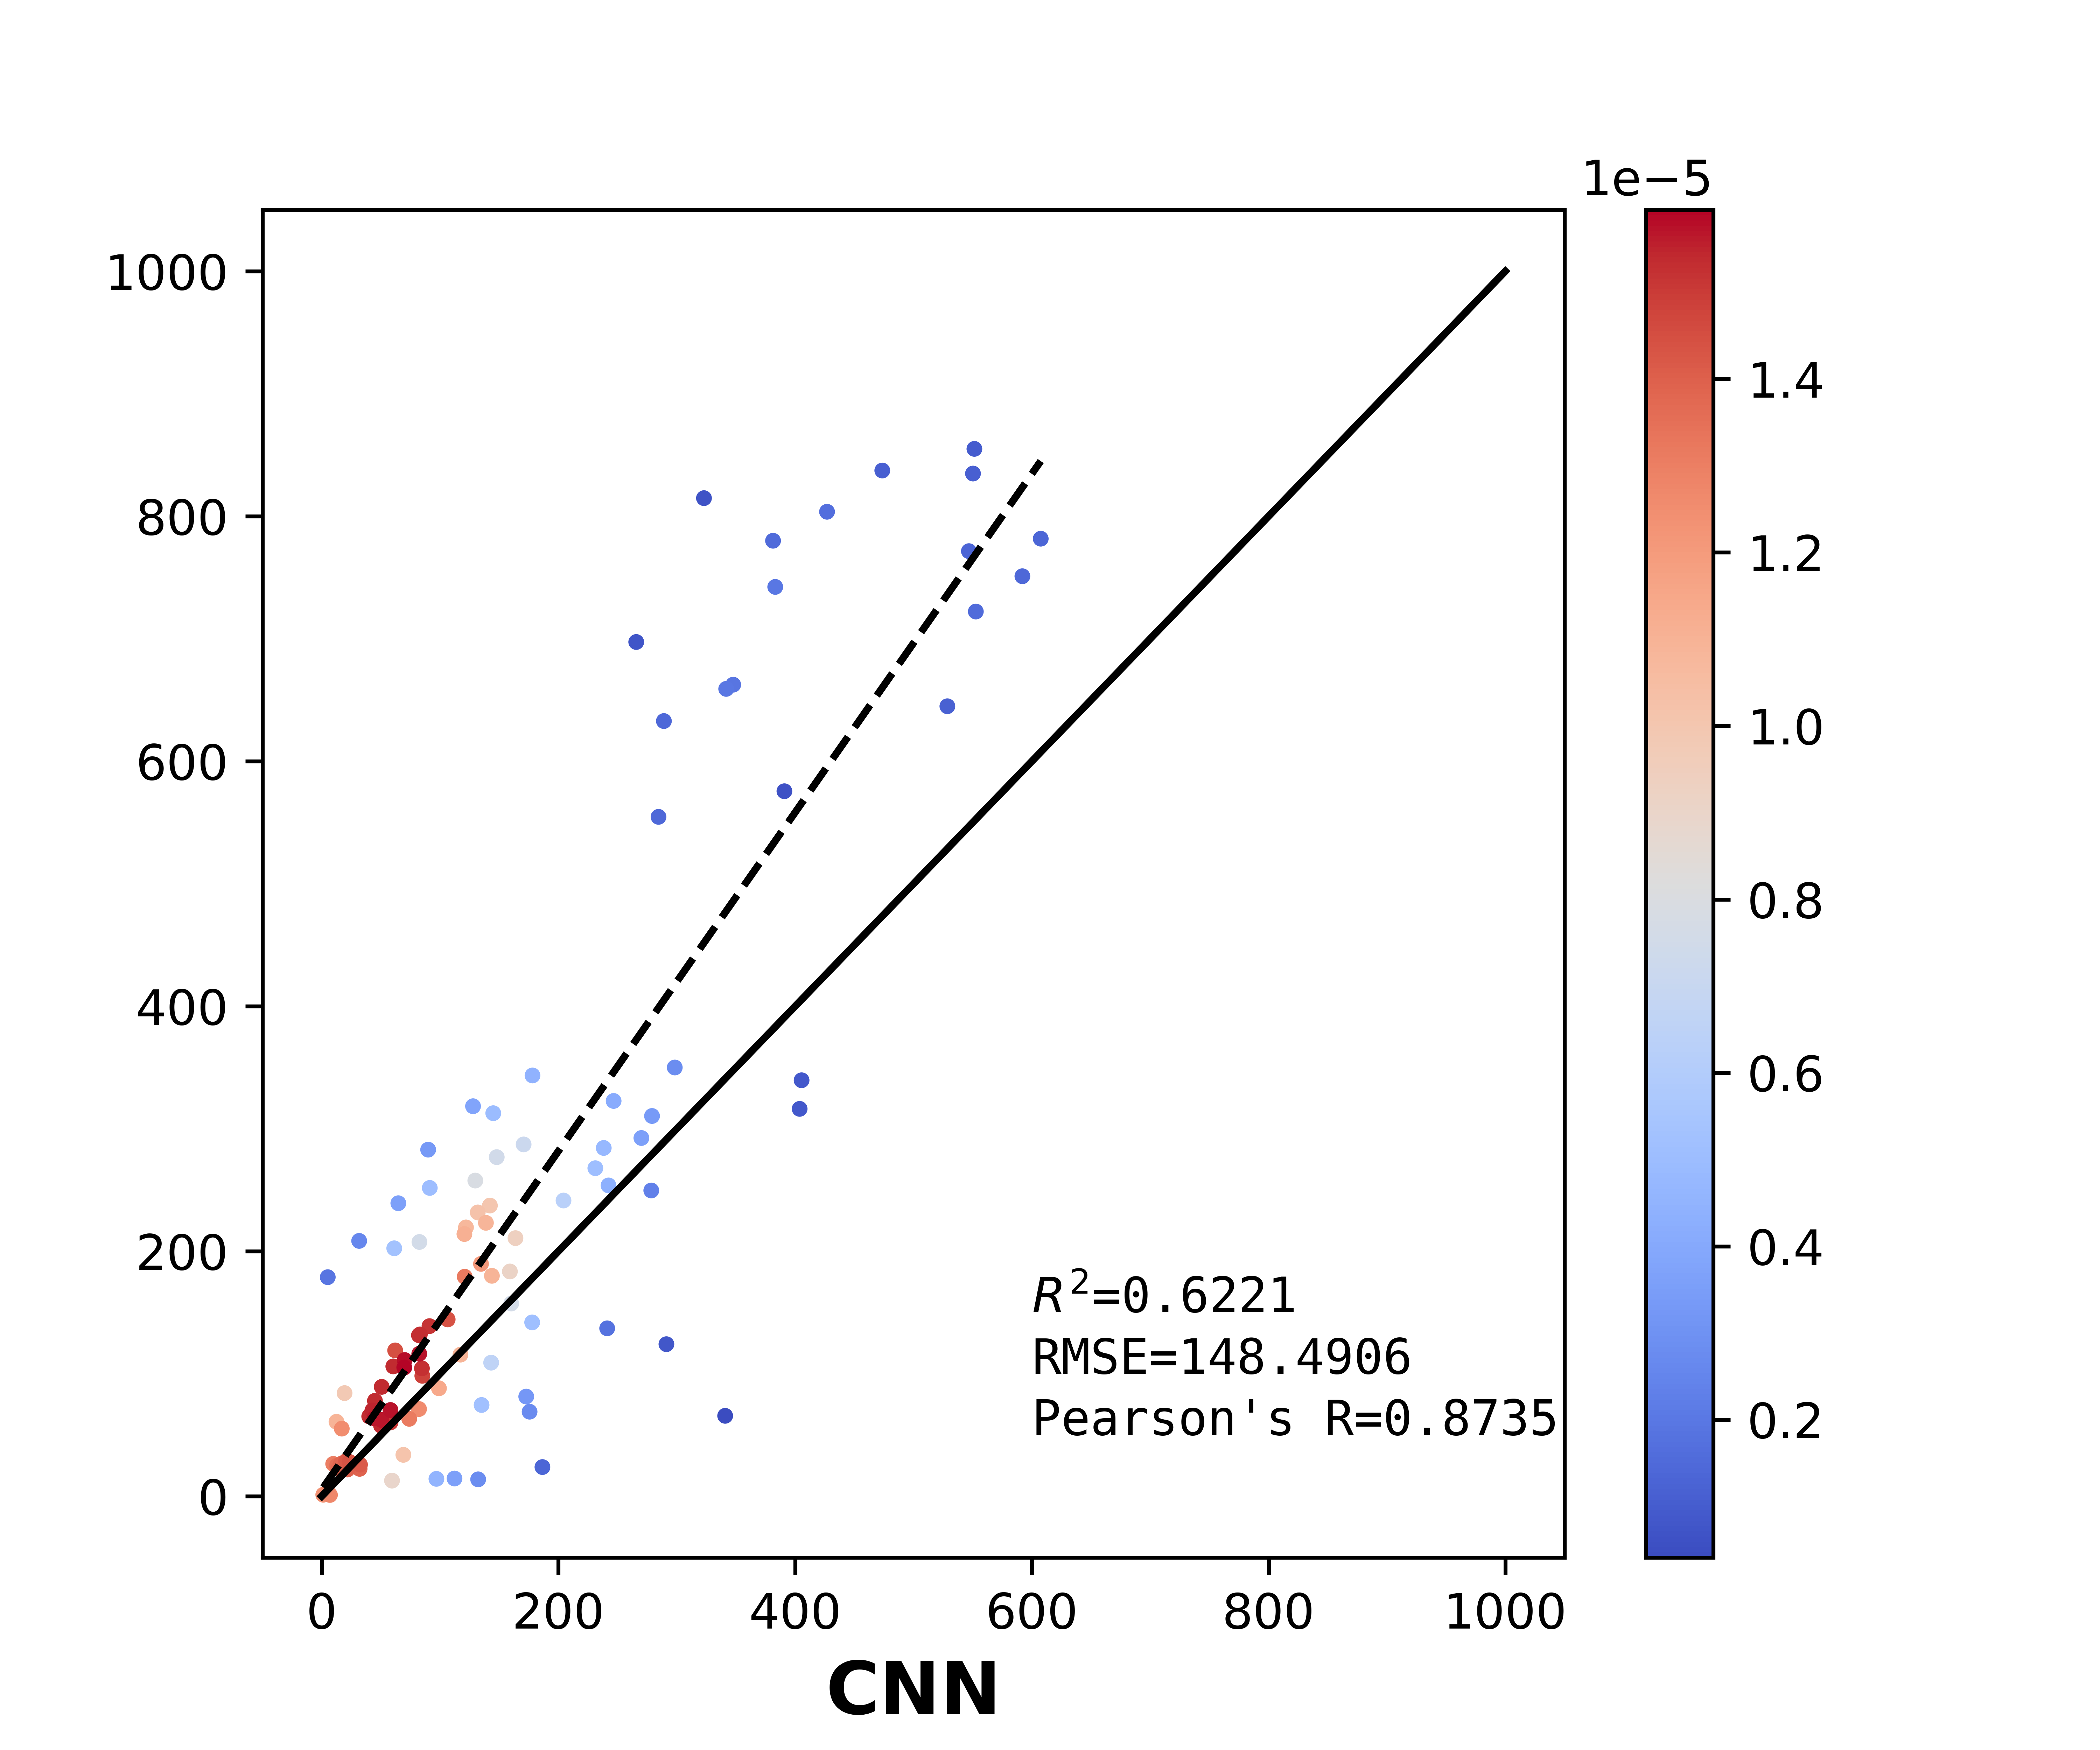
\includegraphics[width=.3\linewidth]{result/cnn_city.png}}\hfill
  \subcaptionbox{DUAL}{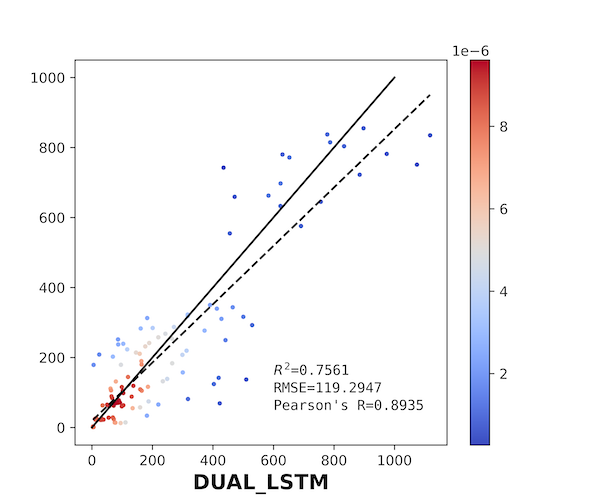
\includegraphics[width=.3\linewidth]{result/dual_city.png}}\hfill
  \subcaptionbox{LSTM}{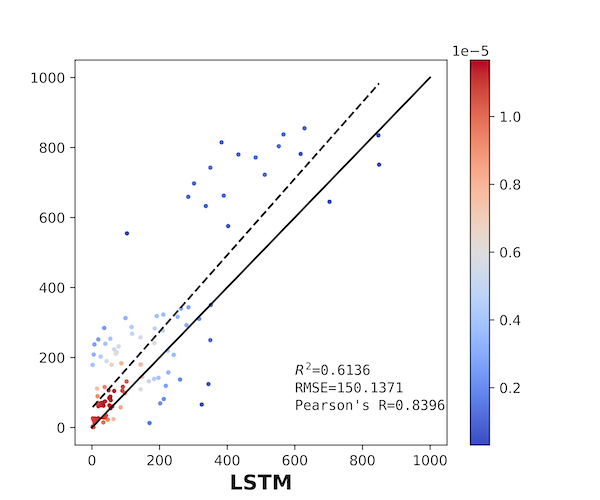
\includegraphics[width=.3\linewidth]{result/lstm_city.png}}\hfill
  \subcaptionbox{RF}{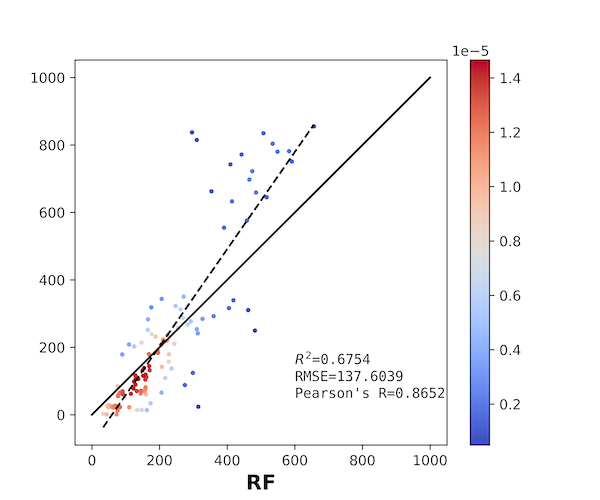
\includegraphics[width=.3\linewidth]{result/rf_city.png}}
  \caption{地级市尺度预估产量与实际产量的散点图}
  \label{fig:scatter_city}
\end{figure}
\begin{figure}
  \centering
  \subcaptionbox{DUAL\_ATT}{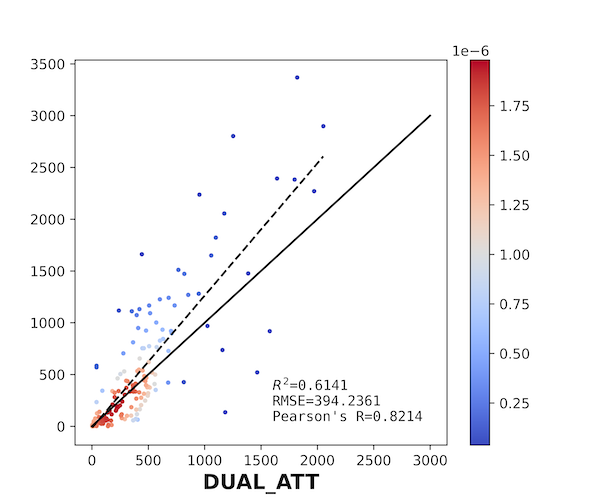
\includegraphics[width=.3\linewidth]{result/dual_att_county.png}}\hfill
  \subcaptionbox{LSTM\_ATT}{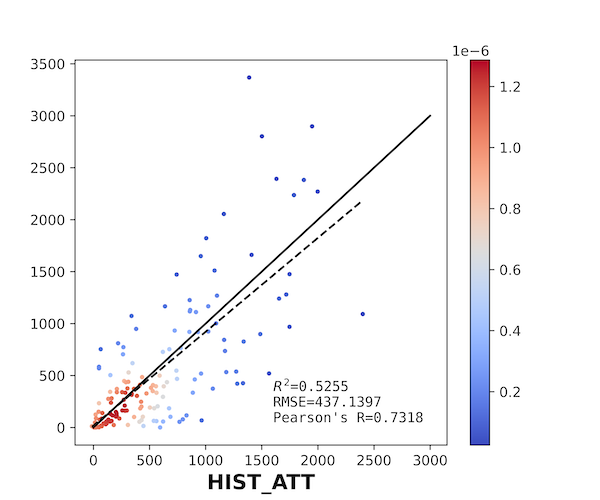
\includegraphics[width=.3\linewidth]{result/lstm_att_county.png}}\hfill
  \subcaptionbox{CNN}{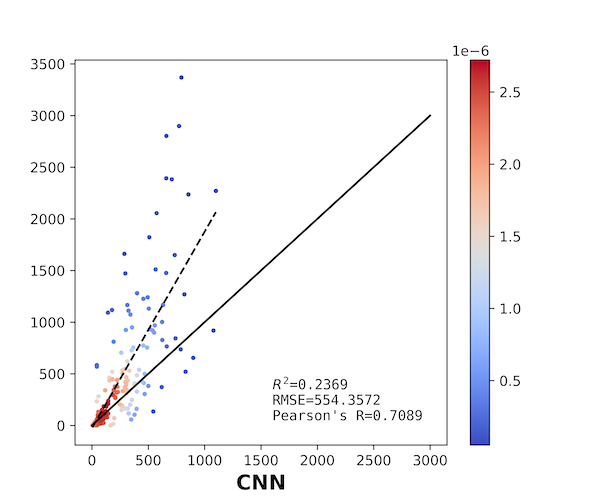
\includegraphics[width=.3\linewidth]{result/cnn_county.png}}\hfill
  \subcaptionbox{DUAL}{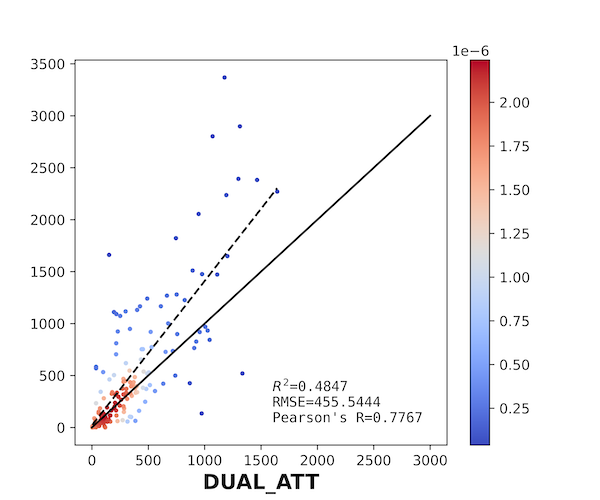
\includegraphics[width=.3\linewidth]{result/dual_county.png}}\hfill
  \subcaptionbox{LSTM}{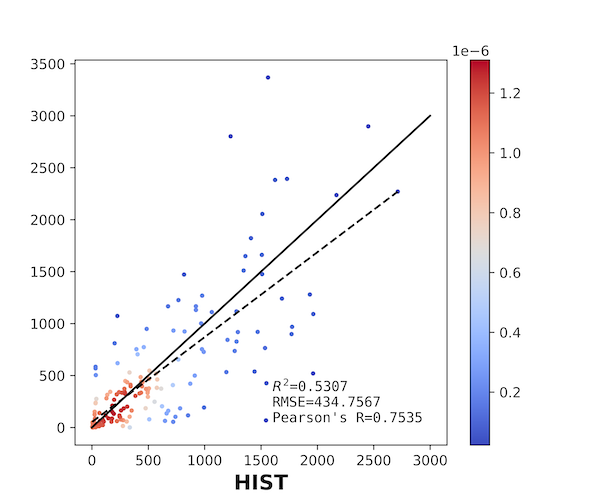
\includegraphics[width=.3\linewidth]{result/lstm_county.png}}\hfill
  \subcaptionbox{RF}{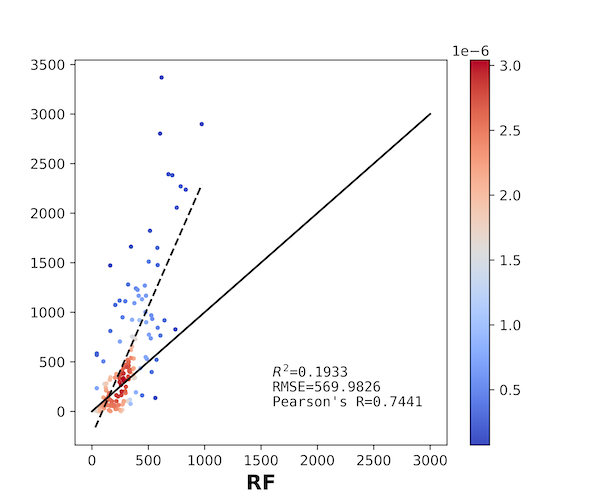
\includegraphics[width=.3\linewidth]{result/rf_county.png}}
  \caption{区县尺度预估产量与实际产量的散点图}
  \label{fig:scatter_county}
\end{figure}

\subsection{误差时空分布分析}

\par 地级市尺度玉米误差分布如\autoref{fig:error_2017}、\autoref{fig:error_2018}和\autoref{fig:error_2019}所示。注意到在地级市尺度上,玉米的误差分布存在着显著的空间差异。其中辽河平原与三江平原地区的误差普遍较低,较大的误差主要出现在以哈尔滨市为中心的松嫩平原地区,且该地区普遍出现了产量低估的现象。分析产量可以发现该地区属于高产量地区,以2019年为例,哈尔滨市、长春市和绥化市的玉米总产量分别为814.78、780.01和722.20万吨。这可能是由于将东北地区划分为地级市尺度后,样本数量相对较少,且高产量地区比例偏低,这导致了在模型训练过程中提取高产量地区作物生长特征的困难,最终导致总产量低估的现象的出现。

\par 对比如\autoref{fig:error_2012}所示的区县尺度玉米误差分布,可以发现该尺度下的误差分布更加均匀,且误差普遍较低。其中,部分缺失真实产量数据的地区使用黄色标记,这些地区主要是城区,其玉米种植面积较小,因此并没有相应的产量数据记录。由于区县尺度下玉米种植面积普遍较小,因此模型在该尺度下的误差分布更加均匀,且误差普遍较低。然而,产量低估的情况依然存在,且在高产量地区更加明显,例如齐齐哈尔市龙江区在2012年的实际产量为336.84万吨,而预估产量仅为182.09万吨。因此,虽然区县尺度下的玉米产量估算具有更好的均匀性和准确性,但仍需要进一步探究和完善估算模型,以更好地解决产量低估问题,特别是在高产量地区。

\begin{figure}
  \centering
  \subcaptionbox{\label{fig:error_2017}2017年地级市尺度误差分布}{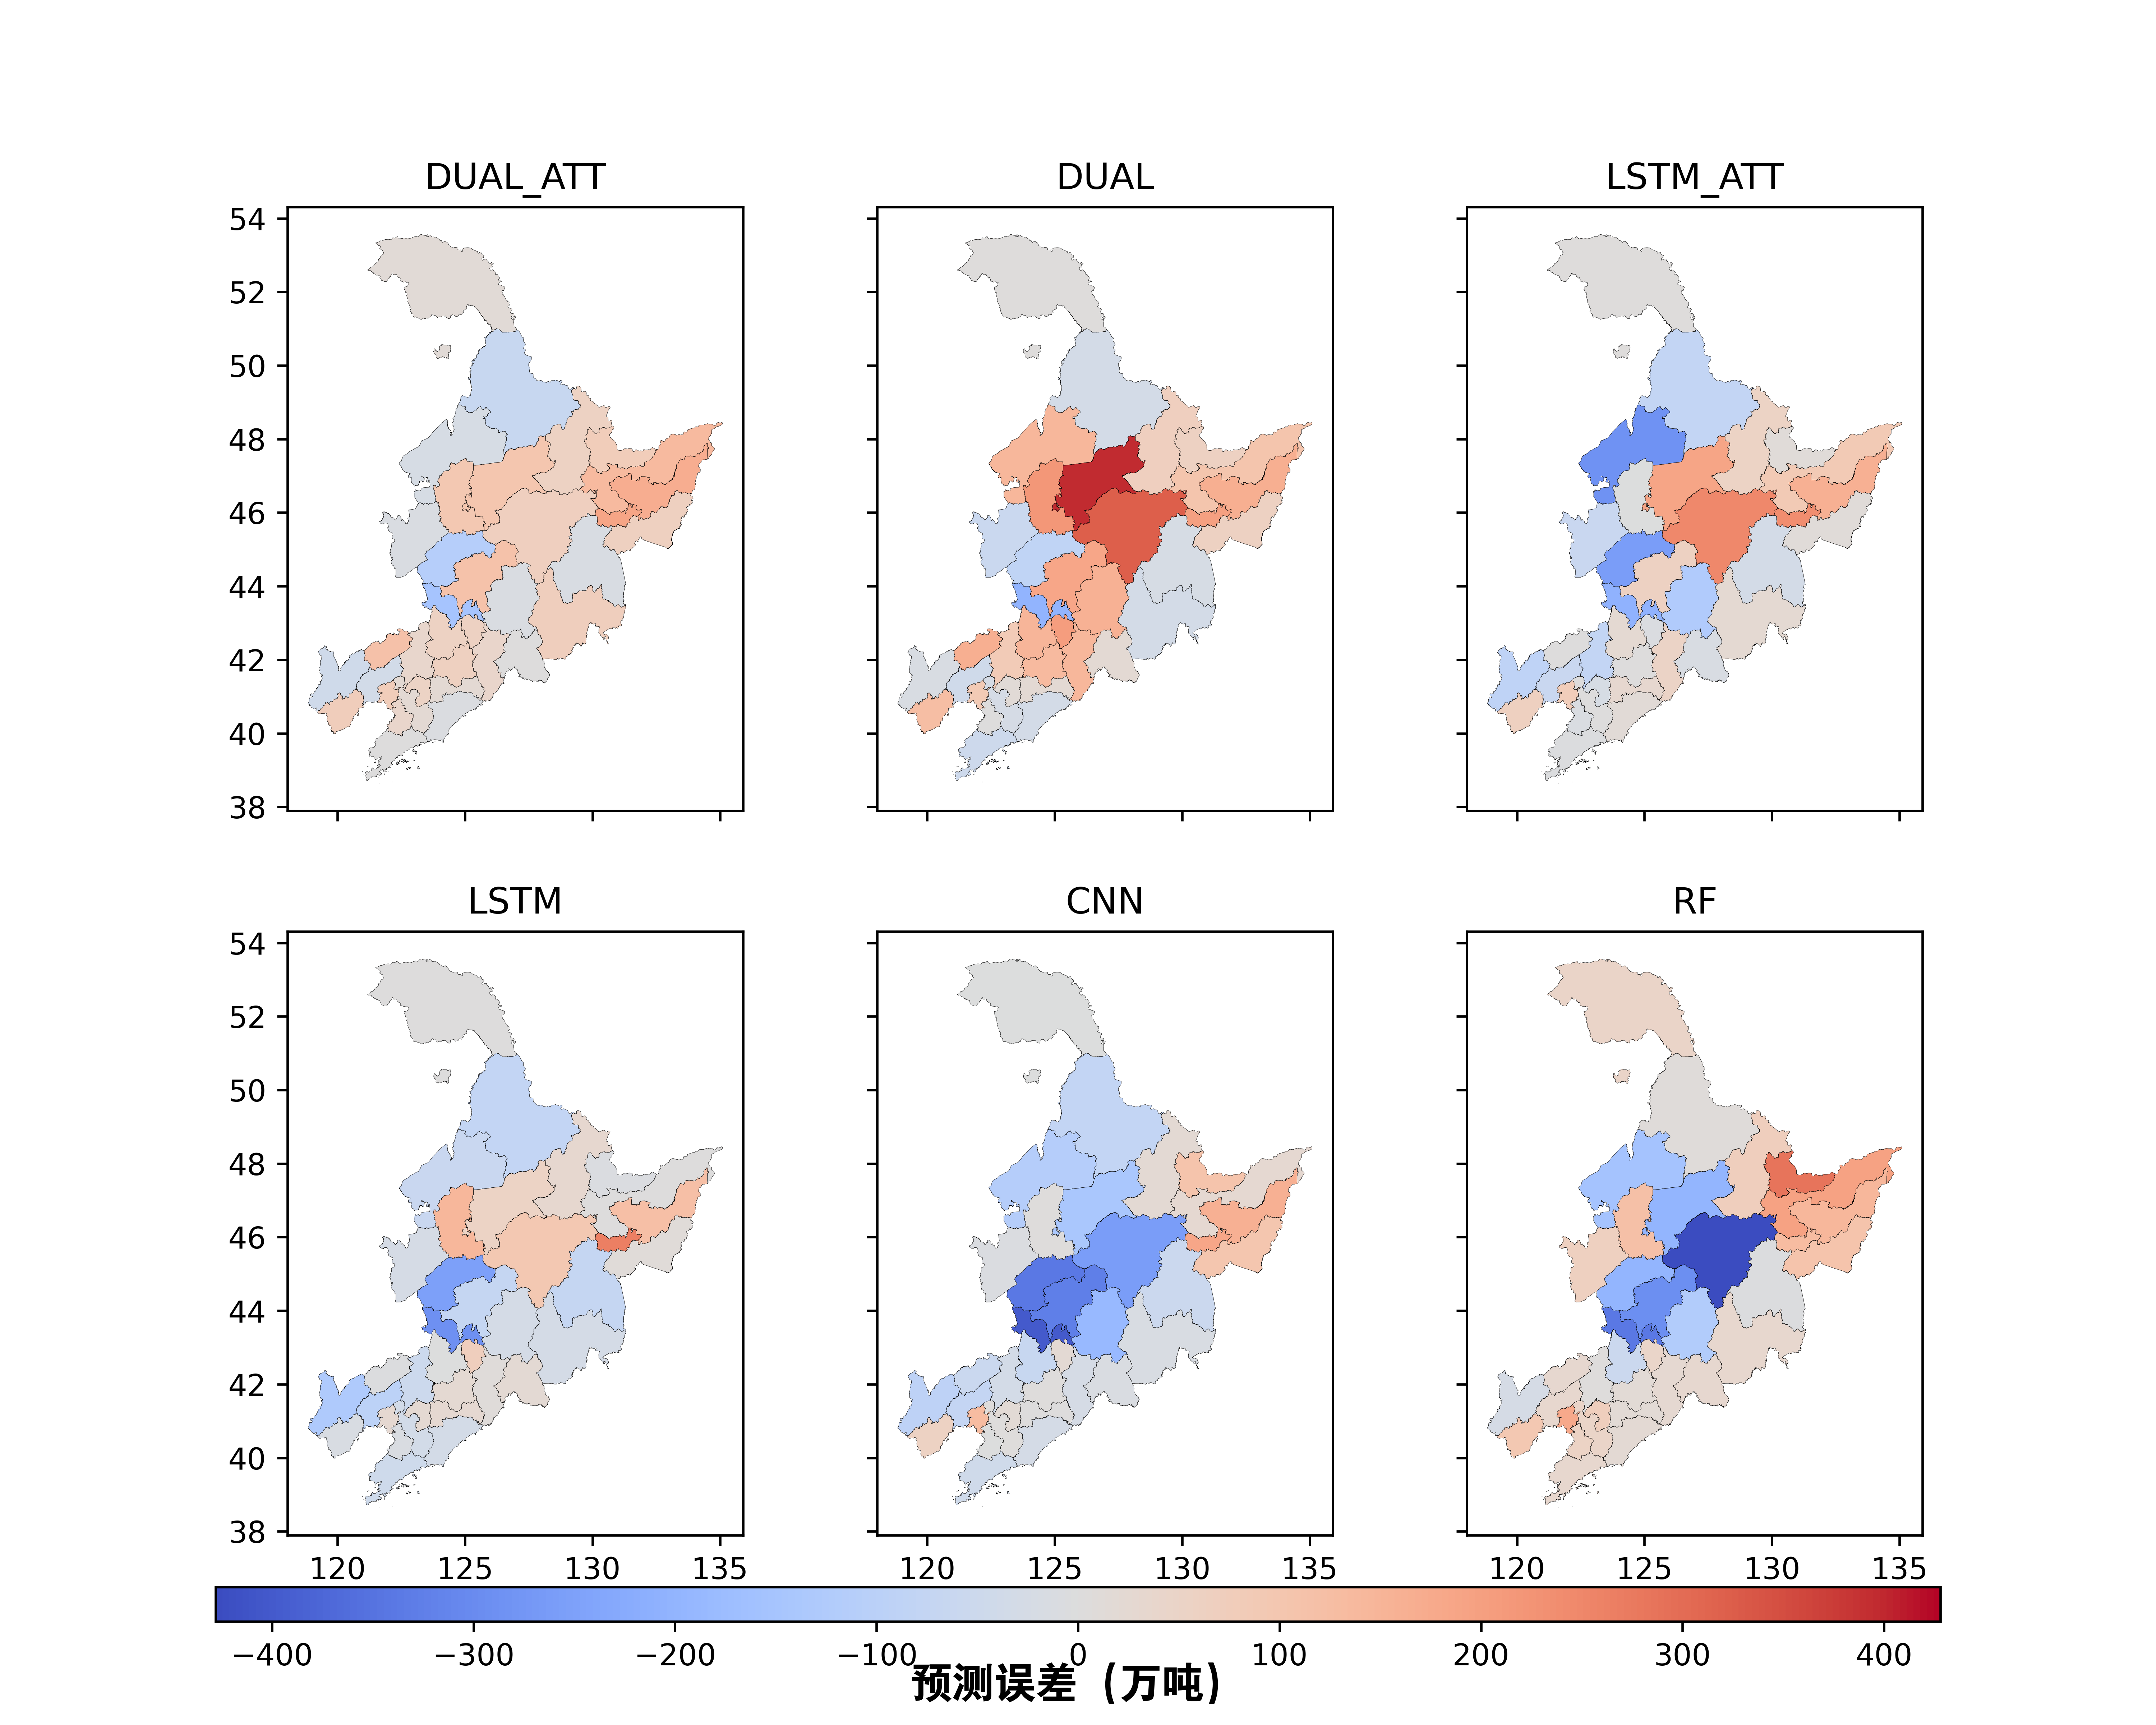
\includegraphics[width=.85\linewidth]{result/error_2017.png}}\hfill
  \subcaptionbox{\label{fig:error_2018}2018年地级市尺度误差分布}{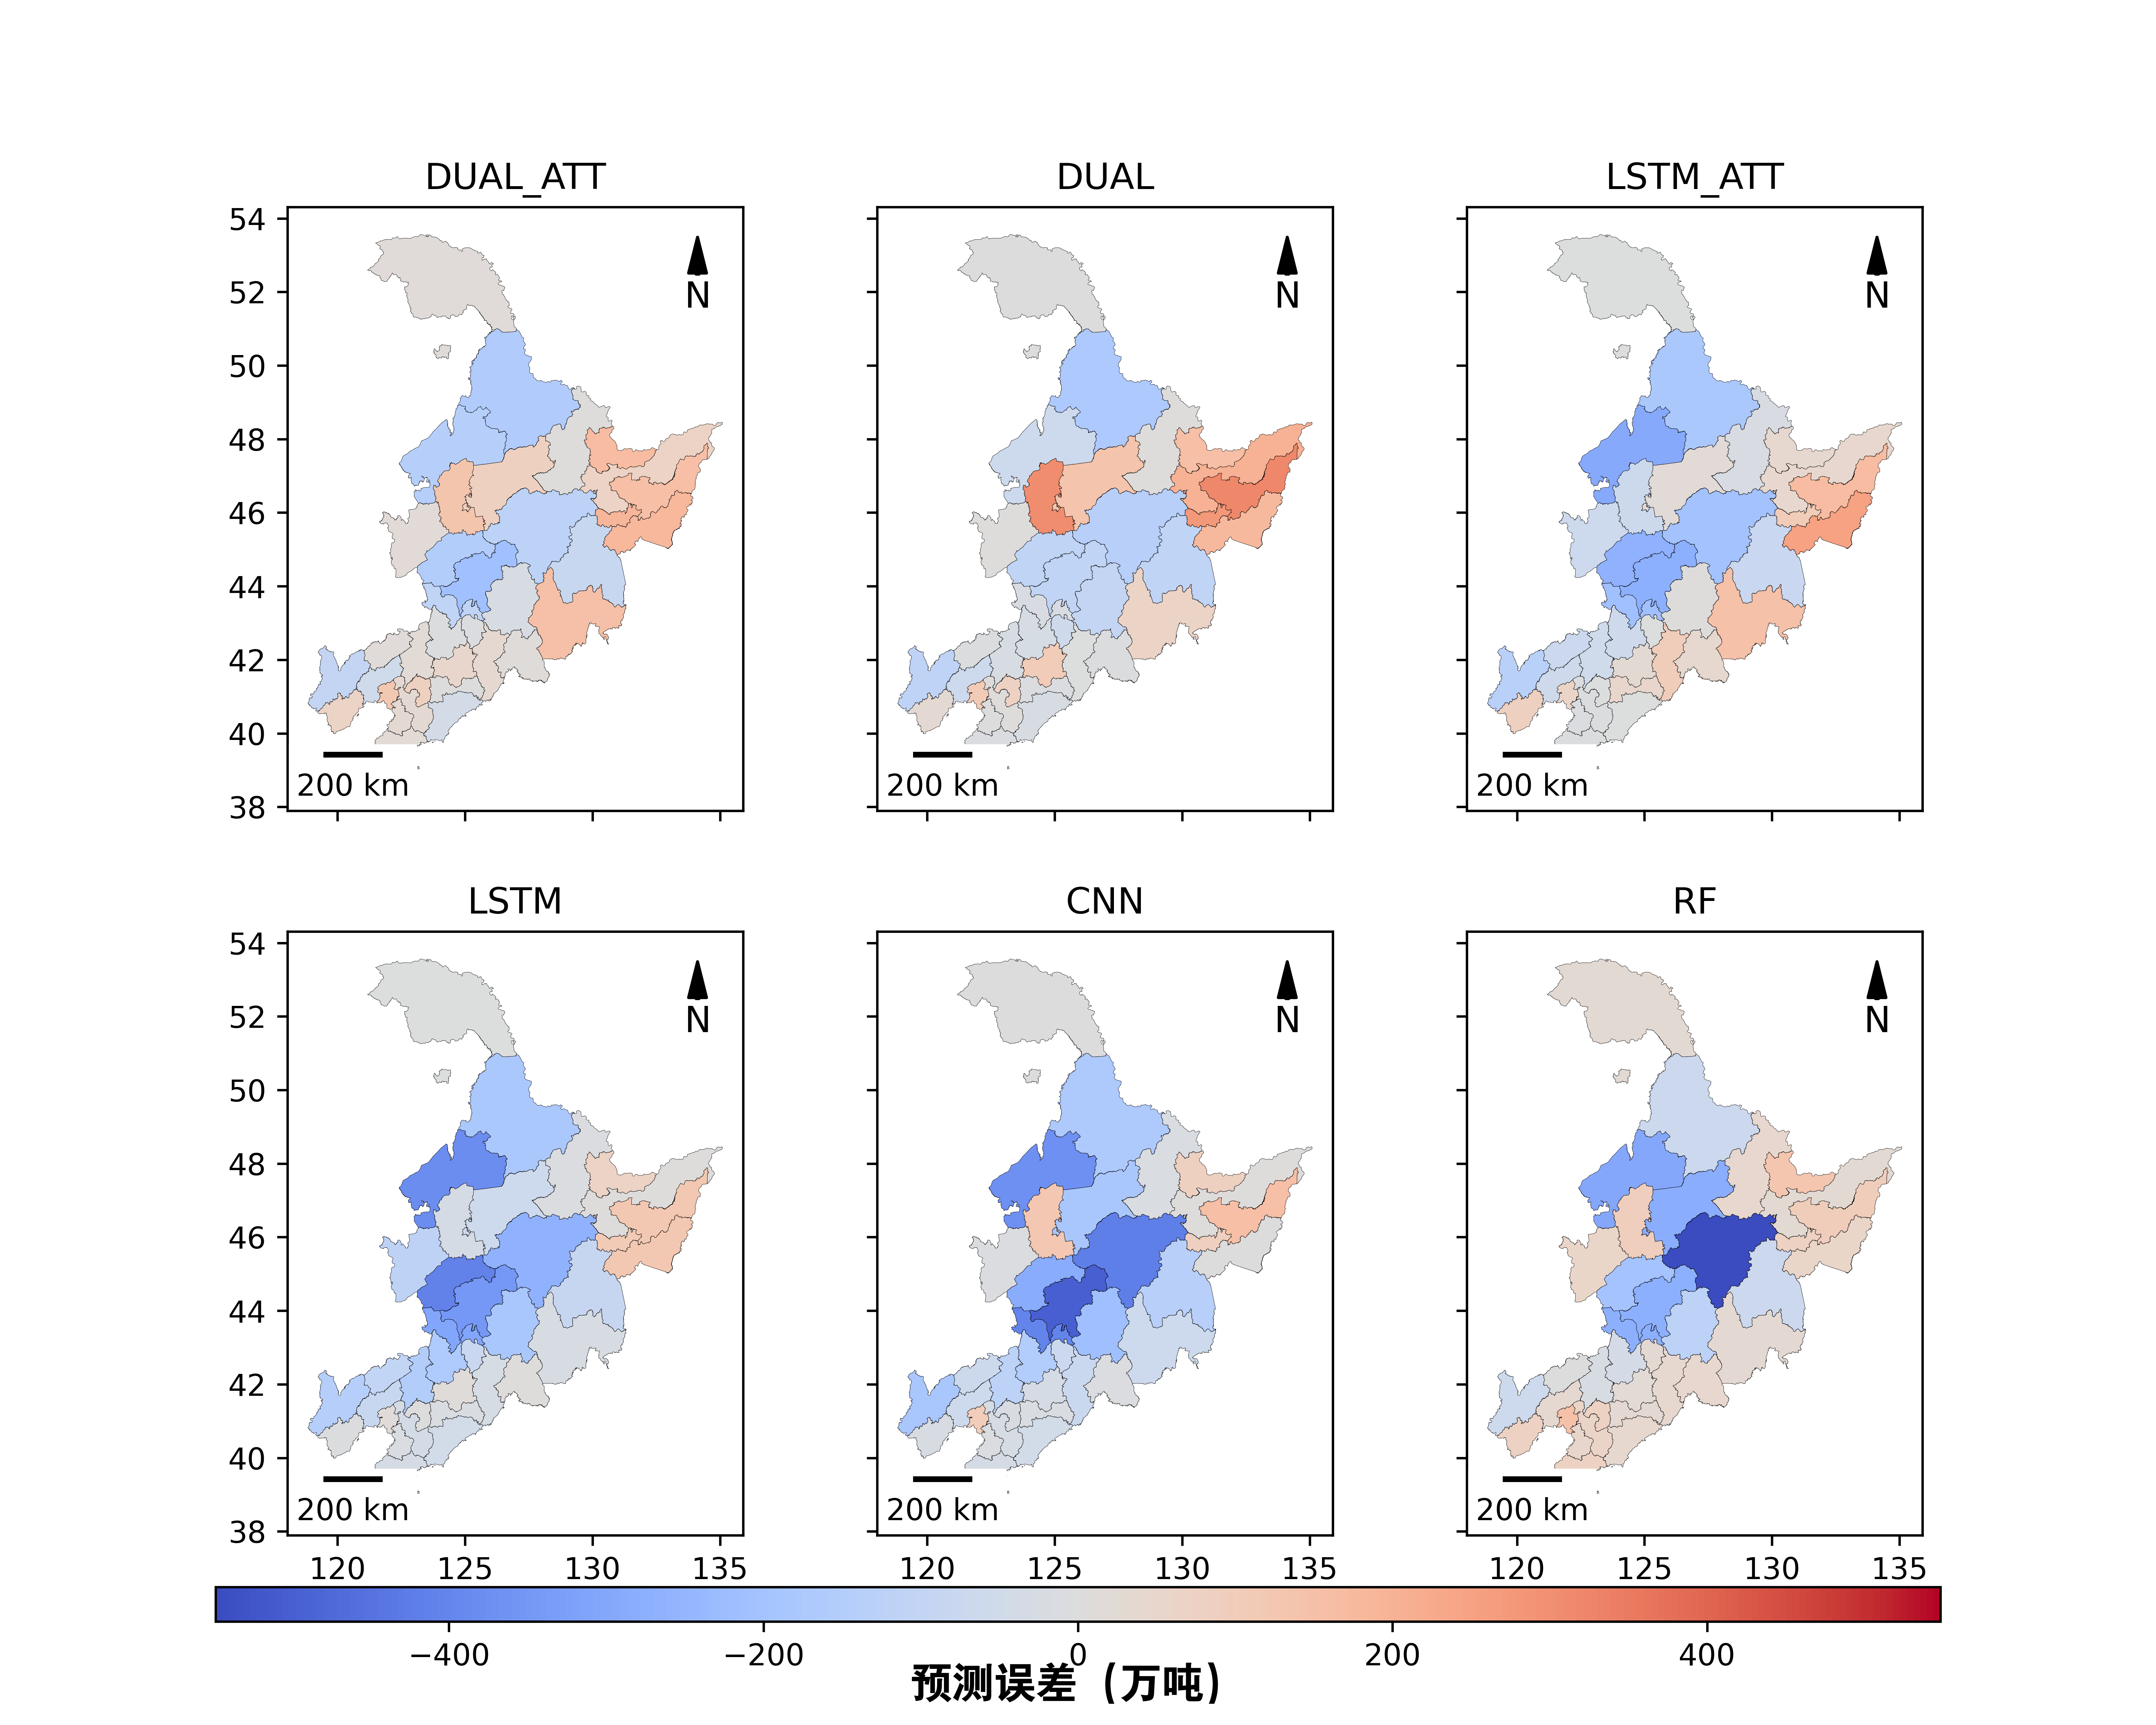
\includegraphics[width=.85\linewidth]{result/error_2018.png}}
\end{figure}
\begin{figure}\ContinuedFloat
  \centering
  \subcaptionbox{\label{fig:error_2019}2019年地级市尺度误差分布}{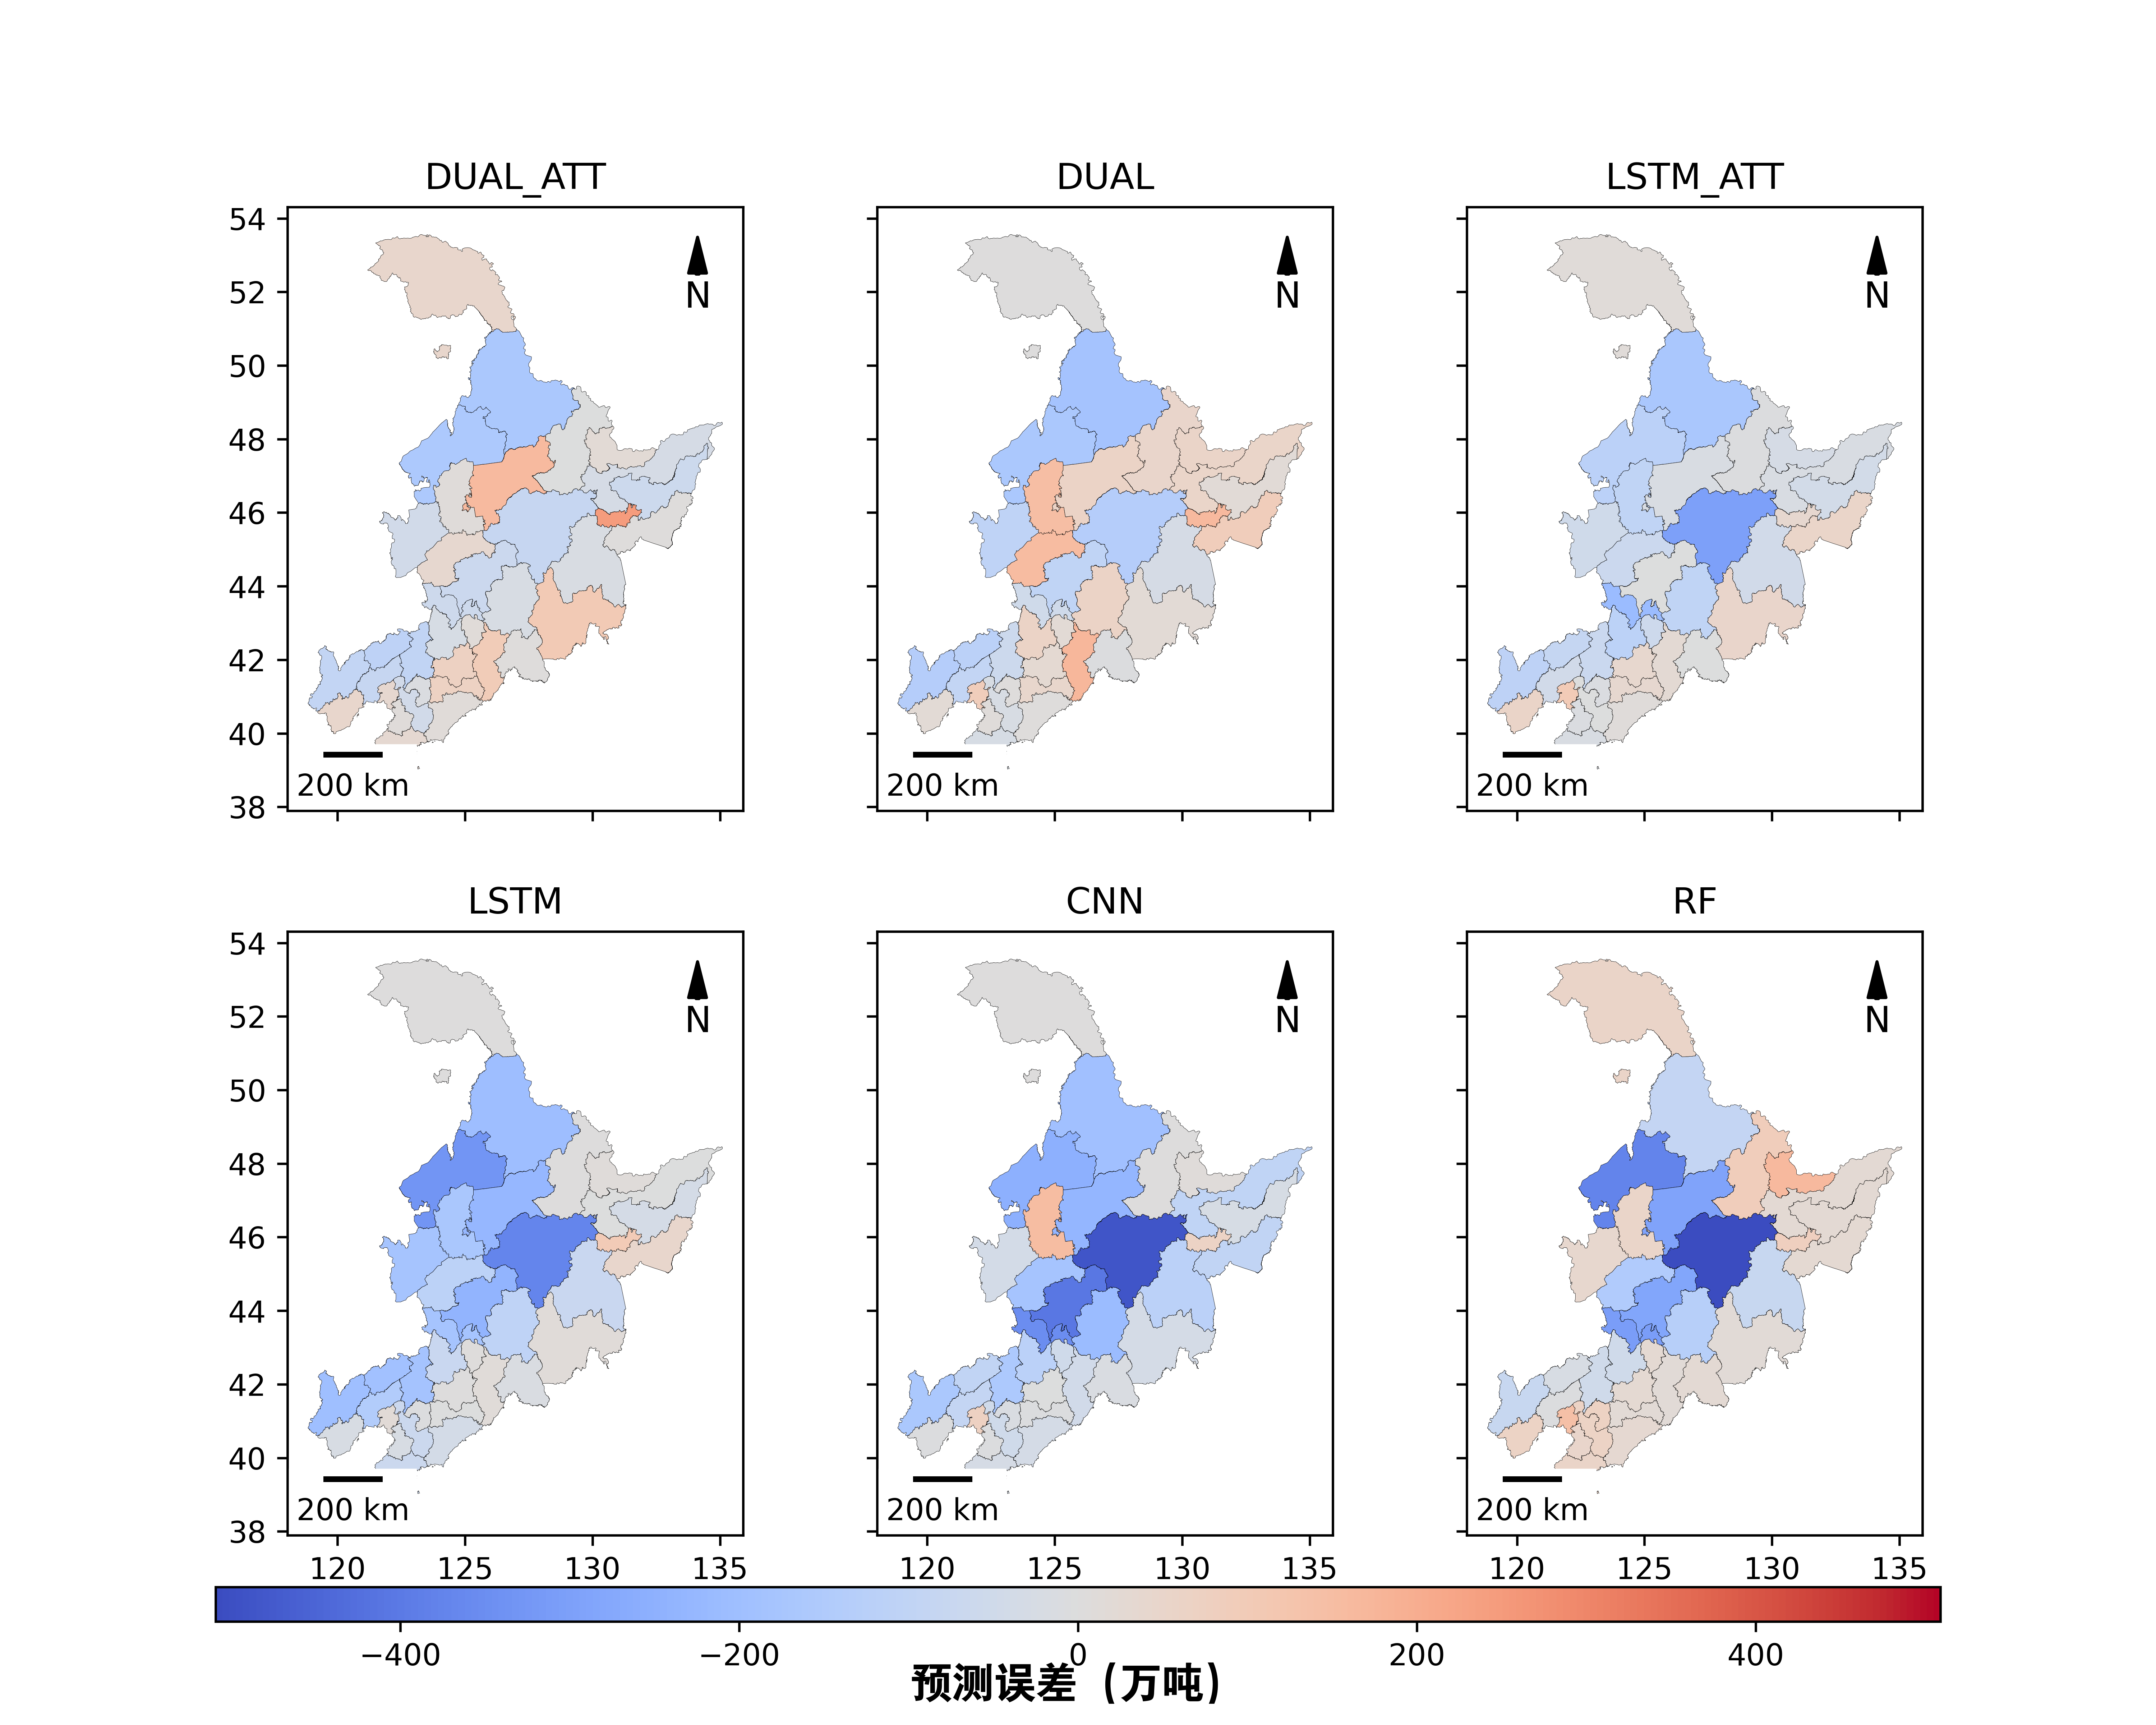
\includegraphics[width=.85\linewidth]{result/error_2019.png}}
  \caption{地级市尺度误差分布}
\end{figure}
\begin{figure}[ht]
  \centering
  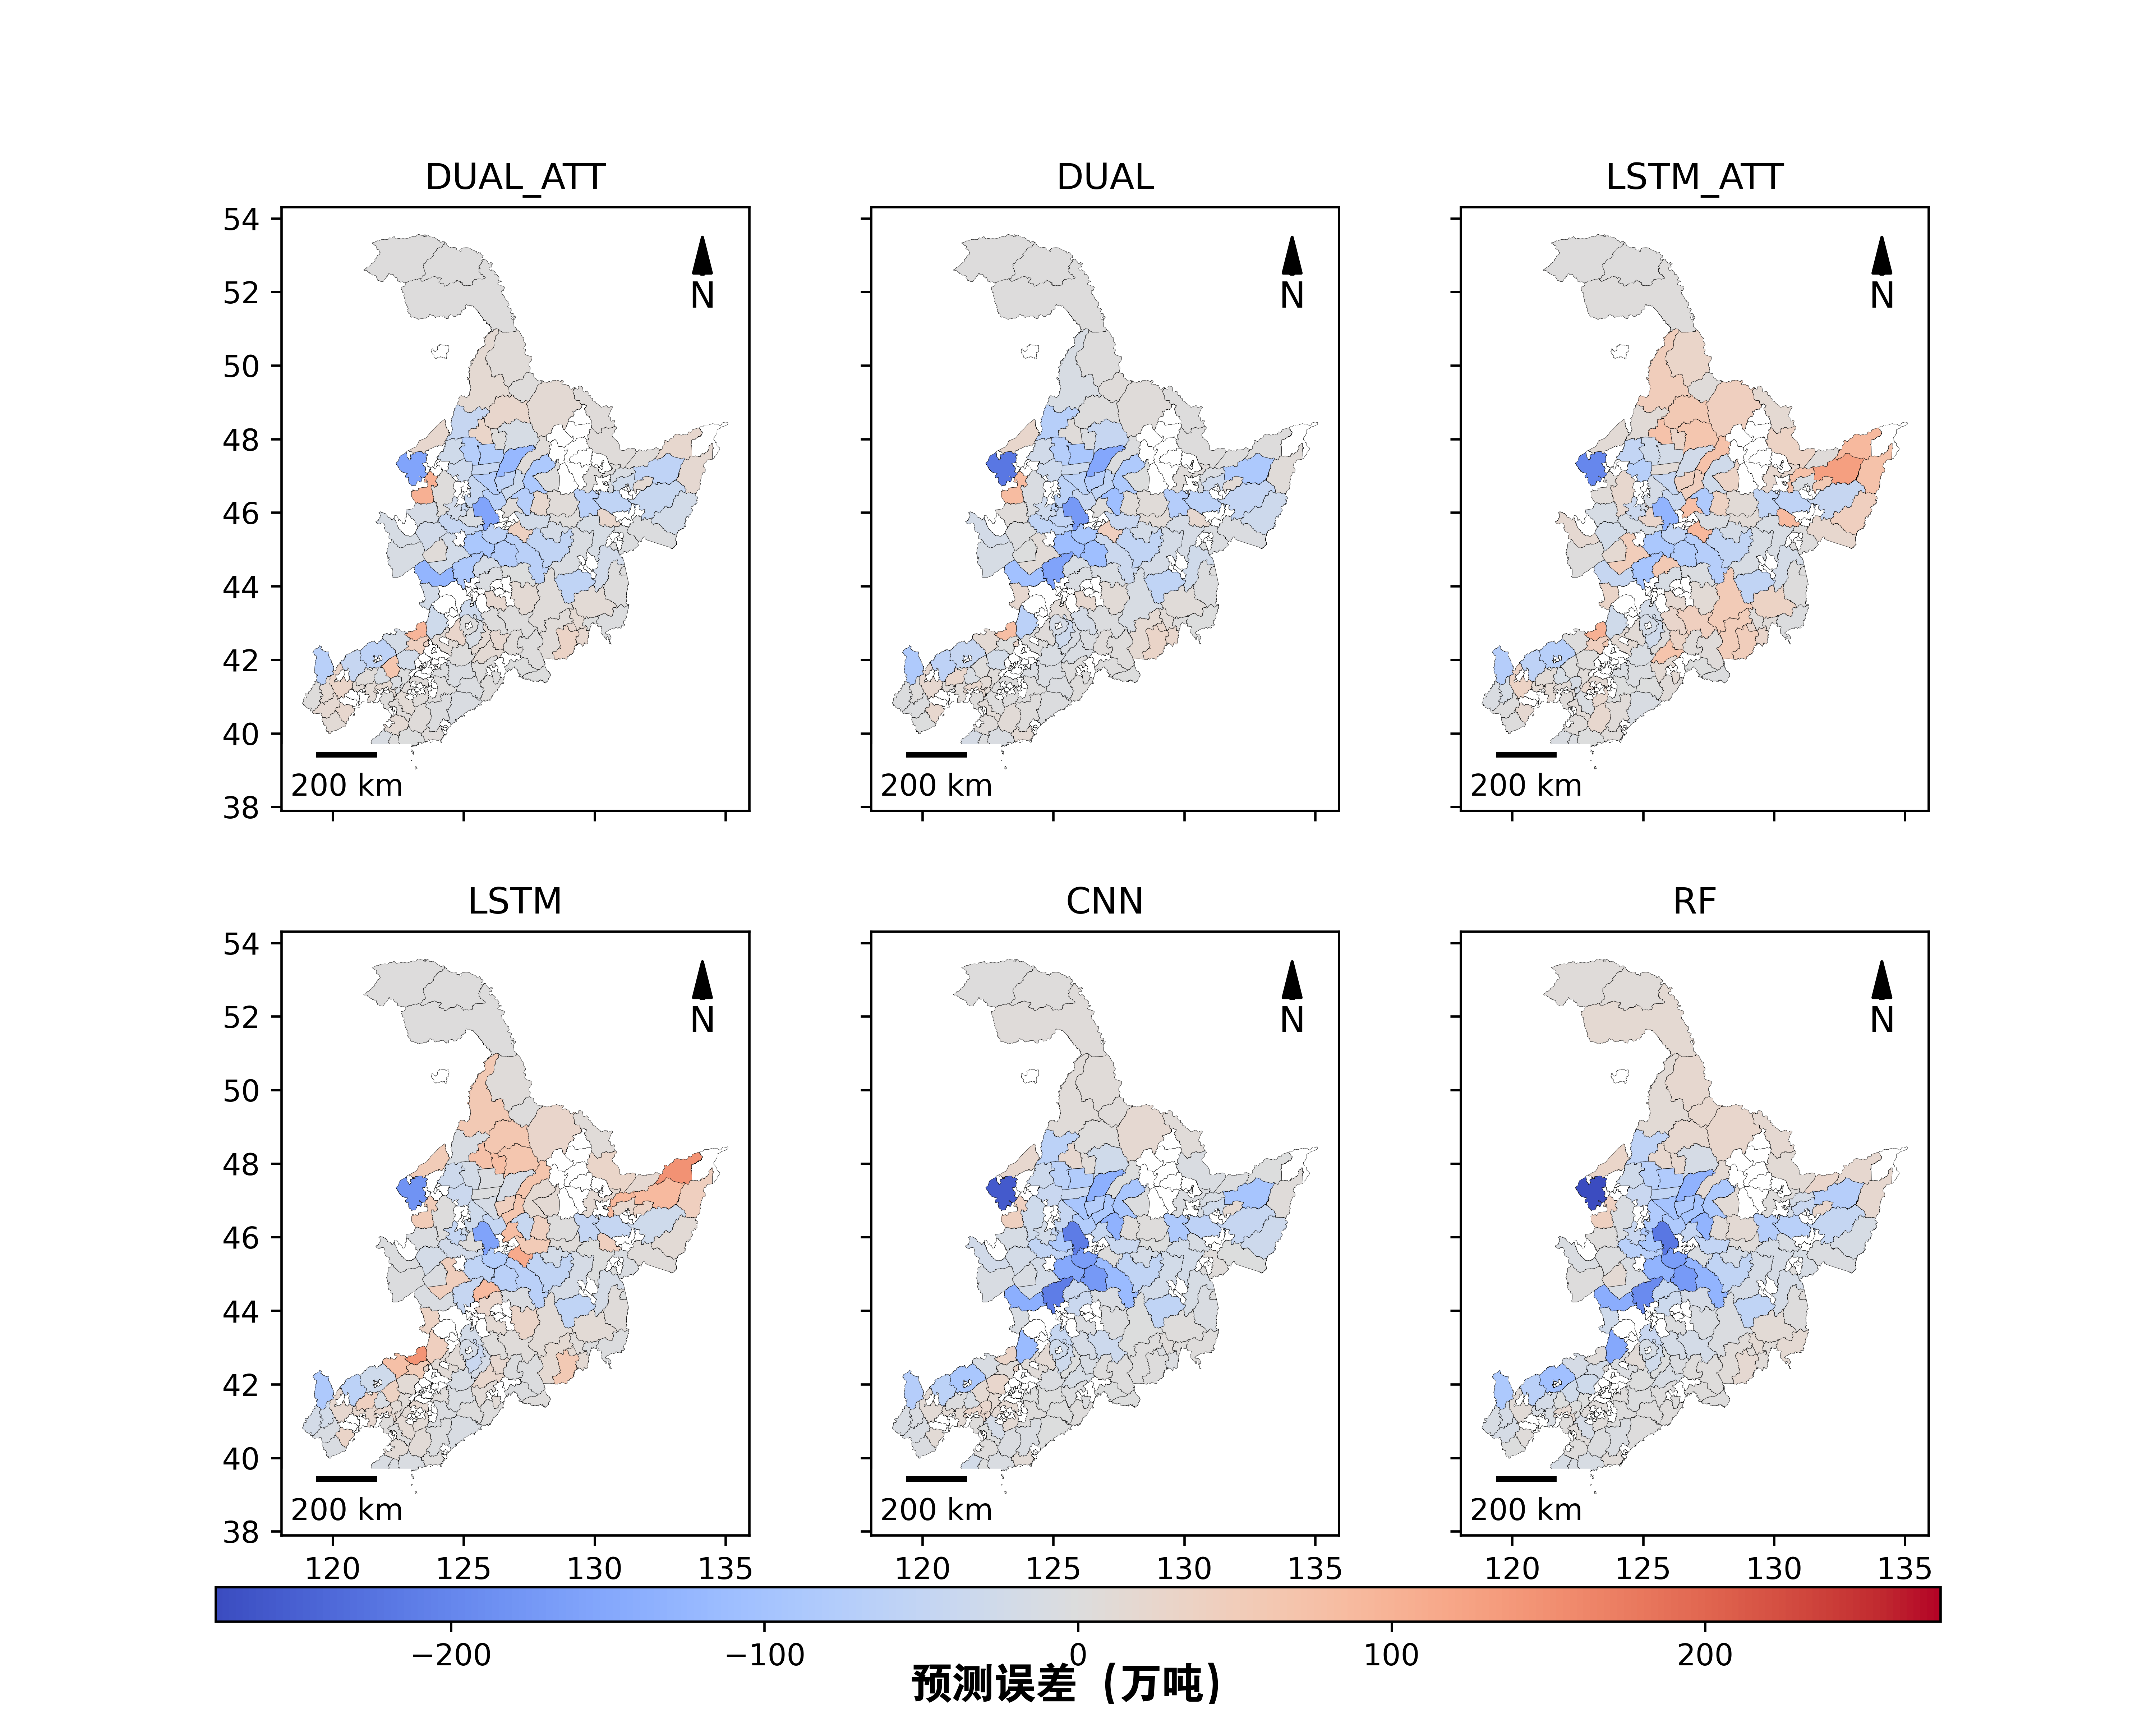
\includegraphics[width=.85\linewidth]{result/error_2012.png}
  \caption{\label{fig:error_2012}2012年区县尺度误差分布}
\end{figure}

\subsection{讨论}
\par 经过实验结果分析可以发现,通过使用直方图采样来降维遥感图像的方法,可以成功地保留作物生长的特征。此外,通过运用了长短期记忆神经网络和注意力机制,研究构建的模型 DUAL\_ATT 能够有效捕捉时间序列中的内在时空关系。这使得模型在地级市和区县尺度上均取得了相较于其他模型更加精确的预估结果。然而,由于数据集的限制,该玉米估产模型在高产量地区仍然出现了产量低估的现象。此外,在模型构建的过程中,研究仅仅使用了 MODIS 遥感产品数据作为输入,并没有考虑其他地面气象数据的辅助,这也可能导致模型在预估玉米产量时受到气象因素的影响,特别是如干旱和洪涝等极端天气事件。因此,在未来的工作中,应该考虑将其他气象数据作为模型的输入,以提高预估的精度。同时也可以考虑对数据集进行进一步的优化,以减少模型出现产量低估的情况。

\par 深度学习模型的训练需要大量的数据集作为基础。然而,囿于国内区域尤其是区县尺度下玉米真实产量数据的获取和验证过程的限制,目前的数据集仍然相对较小。本研究在区县尺度和地级市尺度的数据集分别包含了2335个和646个有效样本,尽管研究采用了多种处理方法提高了数据的精度和质量,但仍需要更多的数据集来进一步验证模型的准确性和泛化能力。由于数据集的局限性,本文的实验仅在东北地区的地级市和县级尺度进行了验证。为了进一步提高模型的泛化能力,未来可以通过收集和处理更多的数据,将模型应用于其他地区,验证模型在不同地区的预测效果。

\par 此外,由于在本研究中所采用的玉米分布数据集 ChinaCropPhen1km 的空间分辨率仅有1km,因此在数据预处理过程中,需要对空间分辨率为500m的 MODIS 产品数据进行重采样,以适应该数据集的空间分辨率。然而,这种重采样可能导致遥感数据信息的缺失,进而影响模型的预估精度。因此,在未来进一步的工作中,我们可以考虑采用更高分辨率的玉米分布数据集,从而更准确地捕捉区域内玉米生长的复杂过程,提高模型的预估精度。

\section{结论与展望}
\par 为了解决大面积作物产量的自适应估计的问题,研究结合了长短期记忆神经网络和注意力机制,以实现作物生长信息的提取,完成区域内的玉米产量估计。研究借助云计算平台 Google Earth Engine 进行遥感数据处理,在地级市和区县两个不同尺度上分别构建了玉米估产模型,高效完成了模型训练和对比测试。主要结论如下:

\begin{itemize}
  \item [(1)] 通过基于长短期记忆神经网络构建的玉米估产模型,研究发现相较于其他对比模型,该方法在大面积作物估产方面有更优秀的表现。在地级市尺度下,该模型取得了更好的预测精度。此外,引入注意力机制后,模型的预测精度进一步提升。
  \item [(2)] 研究采用直方图降维的方式提取作物生长特征。通过这种方法,作物生长信息得到了有效的保留,并使得模型在不同尺度下均有较好的预测效果。
\end{itemize}

\par 在未来的研究工作中,可以继续从数据集的角度进行优化,包括数据量和数据精度的提升,以进一步提高模型的泛化能力。此外,可以考虑将气象数据、作物种植空间分布作为模型的输入,以探究其他因素对于模型精度的影响。